\documentclass[11pt,a4paper]{article}

\usepackage[T1]{fontenc}
\usepackage[utf8]{inputenc}
\usepackage[margin=1.7cm]{geometry}
\usepackage{lmodern}
\usepackage{microtype}
\usepackage{amsmath,amssymb,mathtools}
\usepackage{graphicx}
\usepackage{subcaption}
\usepackage{booktabs}
\usepackage{tabularx}
\usepackage{siunitx}
\usepackage[hidelinks]{hyperref}
\usepackage{enumitem}
\usepackage{placeins}
\usepackage{float}

\graphicspath{{../results/}}
\captionsetup{font=small, labelfont=bf, skip=4pt, hypcap=false}
\setlist[itemize]{leftmargin=*, nosep}
\setlength{\textfloatsep}{7pt plus 2pt minus 2pt}
\setlength{\floatsep}{8pt plus 2pt minus 2pt}
\setlength{\intextsep}{8pt plus 2pt minus 2pt}
\setlength{\abovedisplayskip}{6pt}
\setlength{\belowdisplayskip}{6pt}
\setlength{\abovedisplayshortskip}{4pt}
\setlength{\belowdisplayshortskip}{4pt}
\setlength{\parskip}{2pt}
\setlength{\parindent}{12pt}
\newcolumntype{L}[1]{>{\raggedright\arraybackslash}p{#1}}
\newcolumntype{Y}{>{\raggedright\arraybackslash}X}
\raggedbottom
\renewcommand{\topfraction}{0.94}
\renewcommand{\bottomfraction}{0.88}
\renewcommand{\textfraction}{0.05}
\renewcommand{\floatpagefraction}{0.8}
\setcounter{topnumber}{4}
\setcounter{bottomnumber}{2}
\setcounter{totalnumber}{5}
\sisetup{
  group-digits = false,
  detect-all = true
}

\begin{document}
\begin{center}
{\Large\bfseries Cooperative Kernel Regression\par}
\vspace{0.2em}
{\large Distributed Optimization, Federated Learning, and Differential Privacy\par}
\vspace{0.3em}
{\normalsize Xiangyu Luo \quad Hamza Tarmadi \quad L\'ery Monnerat\par}
\end{center}
\vspace{0.4em}

\section{Introduction}
Kernel regression provides a flexible nonlinear model, but its practical behavior changes substantially once the computation is distributed across communicating agents or clients. The common model considered here is a strongly convex Nystrom approximation of kernel ridge regression, which makes it possible to compare peer-to-peer optimization, federated averaging, and differentially private consensus under the same statistical objective.

The analysis proceeds from the centralized linear system to the local objectives solved by the agents, and then studies how graph topology, local training depth, client heterogeneity, and privacy noise alter convergence. The emphasis is on relating the observed curves to smoothness, strong convexity, and consensus mechanisms rather than on treating the figures as self-contained evidence.

\section{Problem Formulation}\label{sec:formulation}
\subsection{Centralized kernel model}
Let $(x_i,y_i)_{i=1}^n$ denote noisy scalar observations of an unknown one-dimensional function. We use the RBF kernel
\begin{equation}
    k(x,z)=\exp\bigl(-(x-z)^2\bigr),
\end{equation}
and replace the full kernel expansion by a Nystrom approximation over $m$ landmark points $x'_1,\dots,x'_m$. Writing $K_{mm}=[k(x'_p,x'_q)]_{p,q}$ and $K_{nm}=[k(x_i,x'_j)]_{i,j}$, the regularized kernel ridge problem is
\begin{equation}
    \alpha^\star = \arg\min_{\alpha\in\mathbb{R}^m}
    \frac{\sigma^2}{2}\alpha^\top K_{mm}\alpha
    + \frac{1}{2}\lVert y-K_{nm}\alpha\rVert_2^2
    + \frac{\nu}{2}\lVert \alpha\rVert_2^2.
    \label{eq:central-objective}
\end{equation}
Since \eqref{eq:central-objective} is quadratic, the centralized optimizer is the solution of
\begin{equation}
    \bigl(\sigma^2 K_{mm}+K_{nm}^\top K_{nm}+\nu I\bigr)\alpha^\star = K_{nm}^\top y,
    \label{eq:central-linear-system}
\end{equation}
which is exactly the linear system solved in the centralized reference computation.

\subsection{Distributed split and evaluation metrics}
For the distributed experiments, the first dataset is split over $a$ agents. If agent $i$ stores a local feature matrix $M_i$ and labels $y_i$, then the global objective is written as $F(\alpha)=\sum_{i=1}^a f_i(\alpha)$ with
\begin{equation}
    f_i(\alpha)=
    \frac{\sigma^2}{2a}\alpha^\top K_{mm}\alpha
    + \frac{1}{2}\lVert y_i-M_i\alpha\rVert_2^2
    + \frac{\nu}{2a}\lVert \alpha\rVert_2^2.
    \label{eq:local-objective}
\end{equation}
The local Hessian is constant,
\begin{equation}
    H_i = \nabla^2 f_i(\alpha)=\frac{\sigma^2}{a}K_{mm}+M_i^\top M_i+\frac{\nu}{a}I,
\end{equation}
so each $f_i$ is $L_i$-smooth and $\mu_i$-strongly convex with $L_i=\lambda_{\max}(H_i)$ and $\mu_i=\lambda_{\min}(H_i)$. The implementation uses $L_{\max}=\max_i L_i\approx\num{112.73}$ and $\mu_{\min}=\min_i \mu_i\approx\num{0.2000}$ for the baseline Part~I setting. Mean optimality gaps $\frac{1}{a}\sum_i\lVert \alpha_i^t-\alpha^\star\rVert_2$ are reported in Parts~I and~III, whereas Part~II uses the objective error $F(\alpha_t)-F(\alpha^\star)$.

The baseline configuration used throughout most of the report is $(n,m,a)=(100,10,5)$ with $\sigma=0.5$, $\nu=1$, and seed $42$. Every stochastic component (initializations, mini-batches, client sampling, privacy noise) draws from a generator seeded with $42$ plus a fixed experiment-specific offset (a CRC32 checksum of the experiment label), so all reported numbers are reproduced exactly by rerunning the code. The second dataset uses five fixed client blocks of size $20$, while the larger-scale privacy experiment switches to $(n,m,a)=(1000,33,100)$. Table~\ref{tab:setup} collects the notation, datasets, and experiment settings reused below.

\begin{table}[!t]
\centering
\footnotesize
\renewcommand{\arraystretch}{1.08}
\setlength{\tabcolsep}{4pt}
\caption{Notation and experimental settings.}
\label{tab:setup}
\begin{tabularx}{\linewidth}{@{}L{0.12\linewidth}YY@{}}
\toprule
Block & Data and model & Settings and metrics \\
\midrule
Global & RBF kernel $k(x,z)=\exp(-(x-z)^2)$, Nystrom rank $m$, and coefficient vector $\alpha\in\mathbb{R}^m$. & Shared constants are $\sigma=\num{0.5}$, $\nu=\num{1}$, and seed $\num{42}$. The centralized reference solves $(\sigma^2K_{mm}+K_{nm}^\top K_{nm}+\nu I)\alpha^\star=K_{nm}^\top y$. \\
Part I & First dataset; the first $n=\num{100}$ samples are split sequentially across $a=\num{5}$ agents, with $20$ points per agent and $m=\num{10}$ landmarks. & Line, small-world, and complete graphs are tested. The main metric is $\frac{1}{a}\sum_i \lVert \alpha_i^t-\alpha^\star\rVert_2$. The large-$n$ study keeps $m=\lceil \sqrt{n}\rceil$ and a fixed $200$-iteration DGD budget up to $n=\num{30000}$. \\
Part II & Second dataset; five client datasets $(X_i,Y_i)$ of size $20$, with a uniform landmark grid on $[-1,1]$ of size $10$. & FedAvg uses $B\in\{20,15\}$, $C\in\{5,3\}$, and $E\in\{1,5,50\}$ under constant or diminishing rates. The metric is $F(\alpha_t)-F(\alpha^\star)$; SCAFFOLD reuses the same client splits. \\
Part III & First dataset; baseline $(n,m,a)=(100,10,5)$ and larger-scale setting $(1000,33,100)$. & DP-DGD is evaluated for $\epsilon\in\{0.1,1,10\}$ using the theorem-aligned schedules from the course notes and the DP paper. The reported metric is the mean optimality gap, together with finite-horizon privacy audits. \\
\bottomrule
\end{tabularx}
\end{table}


\begin{figure}[!t]
    \centering
    \begin{subfigure}[t]{0.48\linewidth}
        \centering
        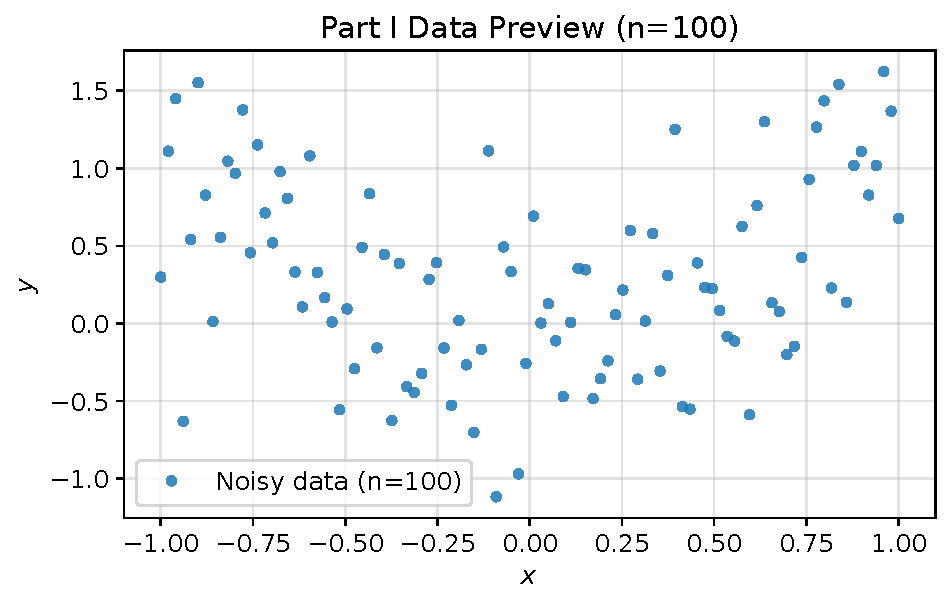
\includegraphics[width=\linewidth]{part1_data_preview.pdf}
    \end{subfigure}\hfill
    \begin{subfigure}[t]{0.48\linewidth}
        \centering
        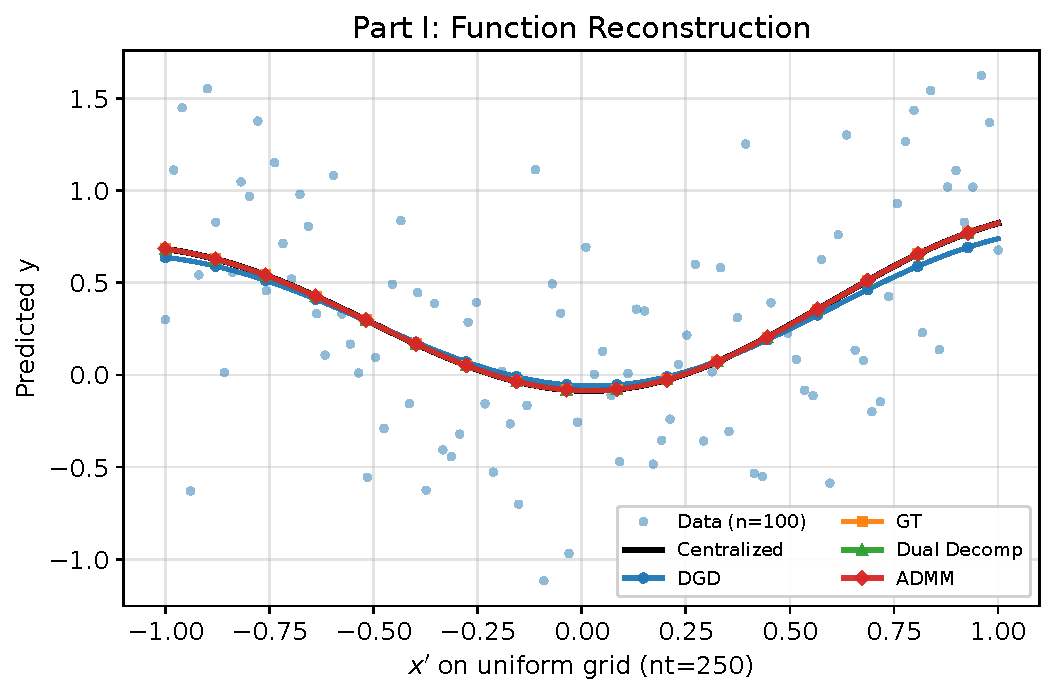
\includegraphics[width=\linewidth]{part1_reconstruction_nt250.pdf}
    \end{subfigure}
    \caption{Data preview and reconstructed functions.}
    \label{fig:preview-reconstruction}
\end{figure}

Figure~\ref{fig:preview-reconstruction} makes two preliminary points that matter later. First, the first dataset is a smooth one-dimensional regression problem with moderate Gaussian noise, so the kernel model is well matched to the data. Second, once training is completed, all distributed solvers reconstruct almost the same function on the 250-point test grid. The main differences observed in Part~I therefore come from optimization speed and consensus accuracy, not from a failure of the regression model itself.

\section{Distributed Optimization}\label{sec:distributed}
\subsection{Algorithms and parameter choices}
The four Part~I solvers correspond directly to the methods covered in Chapters~2 and~4 of the course notes. DGD iterates
\begin{equation}
    x_i^{k+1}=\sum_{j=1}^a w_{ij}x_j^k-\eta\nabla f_i(x_i^k),
\end{equation}
while gradient tracking augments this recursion with a tracker $g_i^k$,
\begin{align}
    x_i^{k+1} &= \sum_j w_{ij}x_j^k-\eta g_i^k,\\
    g_i^{k+1} &= \sum_j w_{ij}g_j^k + \nabla f_i(x_i^{k+1})-\nabla f_i(x_i^k).
\end{align}
Dual decomposition enforces consensus through edge multipliers and the incidence matrix $A$, whereas ADMM alternates local primal updates, edge averages, and dual corrections. Because the local objectives are quadratic, all step-size checks can be carried out directly from the stored Hessians and graph matrices. This is especially useful for GT, where the linearized stacked dynamics can be checked through the spectral radius of the reduced transition matrix. Table~\ref{tab:theory} summarizes the implemented hyperparameters and the corresponding theory checks.

\begin{table}[!htb]
\centering
\scriptsize
\renewcommand{\arraystretch}{1.02}
\setlength{\tabcolsep}{3.2pt}
\caption{Parameter choices and checks; lecture-note bounds are used except for the DP schedule, which follows Wang--Nedic Theorem~2(3).}
\label{tab:theory}
\begin{tabularx}{\linewidth}{@{}L{0.10\linewidth}L{0.18\linewidth}L{0.23\linewidth}Y@{}}
\toprule
Method & Principle & Choice & Check \\
\midrule
DGD & Smooth bound $O(1/L)$. & $\eta_{\mathrm{DGD}}=0.2/L_{\max}$. & $L_{\max}=\num{1.12726e+02}$ and $\eta_{\mathrm{DGD}}=\num{1.77421e-03}<2/L_{\max}=\num{1.77421e-02}$; the baseline run is stable on all three undirected graphs. \\
GT & Spectral-radius test. & $\eta_{\mathrm{GT}}=0.6/L_{\max}$. & $\rho(T(\eta_{\mathrm{GT}}))=\num{9.98935e-01}<1$, with a scanned threshold near $\num{6.13375e-03}$; the method remains accurate across graph topologies. \\
Dual & Dual-ascent bound. & $\eta_{\mathrm{dual}}=0.9\cdot 2\mu_{\min}/\sigma_{\max}(A)^2$. & $\mu_{\min}=\num{2.00000e-01}$, $\sigma_{\max}(A)=\num{1.90211e+00}$, and $\eta_{\mathrm{dual}}=\num{9.95016e-02}<\num{1.10557e-01}$; the line-graph gap reaches the \num{1e-6} range. \\
ADMM & Positive-penalty condition. & $\beta\in\{0.1,1,10,100\}$. & All tested penalties are admissible; $\beta=1$ and $\beta=10$ are the fastest practical choices. \\
FedAvg & Smooth SGD bound. & $\eta_0=\num{2.000e-03}$ and $\eta_t=0.002/(1+0.01t)$. & $L_{\max}^{\mathrm{FL}}=\num{7.97264e+01}$ and $\eta_0<2/L_{\max}^{\mathrm{FL}}=\num{2.50858e-02}$; $E=50$ gives the best final error in both learning-rate schedules. \\
SCAFFOLD & Control-variate correction. & Constant local rate $\eta=\num{2e-3}$, matched to FedAvg. & With the same local rate, the corrected runs outperform FedAvg at $E=50$ for both $C=5$ and $C=3$. \\
DP-DGD & Summability conditions. & $\alpha_k=\frac{0.002}{1+0.001k}$, $\gamma_k=\frac{1}{1+0.001k^{0.9}}$, $\nu_k=\frac{0.01}{\epsilon}\bigl(1+0.001k^{0.1}\bigr)$. & On $3000$ steps, $\sum \alpha_k^2/\gamma_k=\num{4.24840e-03}$ and $\sum \alpha_k/\nu_k|_{\epsilon=1}=\num{2.76645e+02}$; smaller $\epsilon$ yields larger final gaps. \\
\bottomrule
\end{tabularx}
\end{table}


\subsection{Convergence under graph constraints}

\paragraph{Line graph.}
The first benchmark uses a line graph with $a=5$ agents. Figure~\ref{fig:line-convergence} shows the resulting convergence curves. After $3000$ iterations, DGD stops at a mean optimality gap of \num{1.4853e-1}, GT reaches \num{8.5918e-4}, dual decomposition reaches \num{4.1365e-6}, and ADMM with $\beta=1$ reaches \num{1.9948e-14}. The ordering is the one expected from theory. DGD with a fixed step converges only to a neighborhood whose size depends on the step and on the graph mixing factor. GT removes that steady-state bias in the strongly convex setting. Dual decomposition and ADMM instead solve exact consensus reformulations, so the iterates can drive the consensus error essentially to machine precision.

\paragraph{Penalty selection.}
The ADMM penalty controls the balance between local objective minimization and consensus enforcement. Figure~\ref{fig:admm-beta} shows that all positive penalties are admissible, but only a moderate range is efficient in finite time: $\beta=1$ and $\beta=10$ both reach machine precision, while $\beta=0.1$ and $\beta=100$ remain visibly slower at the same horizon. This behavior is typical of quadratic consensus problems, where overly small penalties weaken the coupling and overly large penalties overemphasize the constrained subproblem.

\noindent
\begin{minipage}[t]{0.49\linewidth}
    \centering
    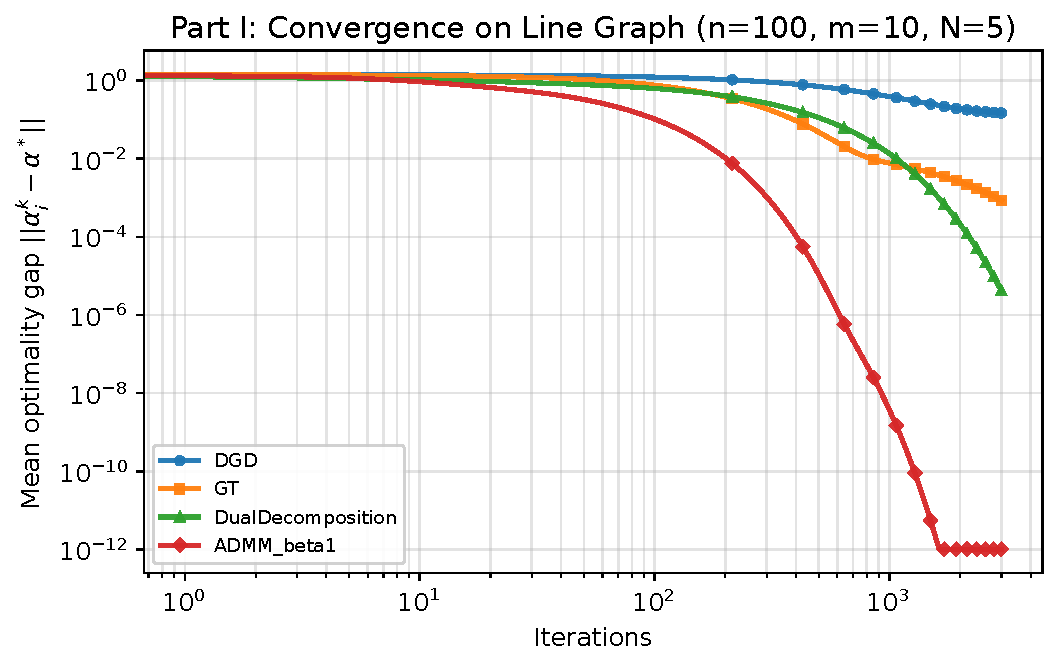
\includegraphics[width=\linewidth]{part1_algorithms_line_loglog.pdf}
\par\smallskip
    \refstepcounter{figure}\label{fig:line-convergence}
    {\small\textbf{Figure \thefigure.} Line-graph convergence.\par}
\end{minipage}\hfill
\begin{minipage}[t]{0.49\linewidth}
    \centering
    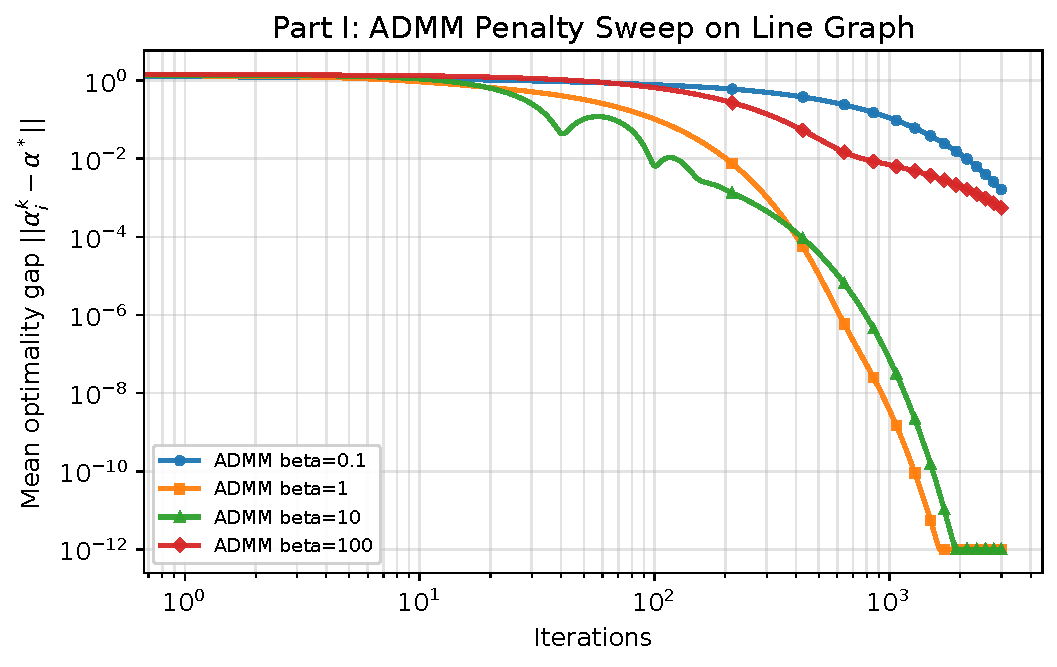
\includegraphics[width=\linewidth]{part1_admm_beta_sweep.pdf}
\par\smallskip
    \refstepcounter{figure}\label{fig:admm-beta}
    {\small\textbf{Figure \thefigure.} ADMM penalty sweep.\par}
\end{minipage}

\paragraph{Graph topology.}
The role of connectivity is separated in Figure~\ref{fig:graph-topology}. For DGD, denser communication clearly helps: the final gap decreases from \num{1.4832e-1} on the line graph to \num{1.3767e-1} on the small-world graph and to \num{7.0235e-2} on the complete graph. For GT, the three curves are much closer, all remaining of order \num{1e-3}. This is precisely what the theory predicts: DGD is strongly affected by the spectral gap of the mixing matrix, while GT is much less sensitive once the exact-tracking mechanism is in place.

\begin{figure}[!htb]
    \centering
    \begin{subfigure}[t]{0.48\linewidth}
        \centering
        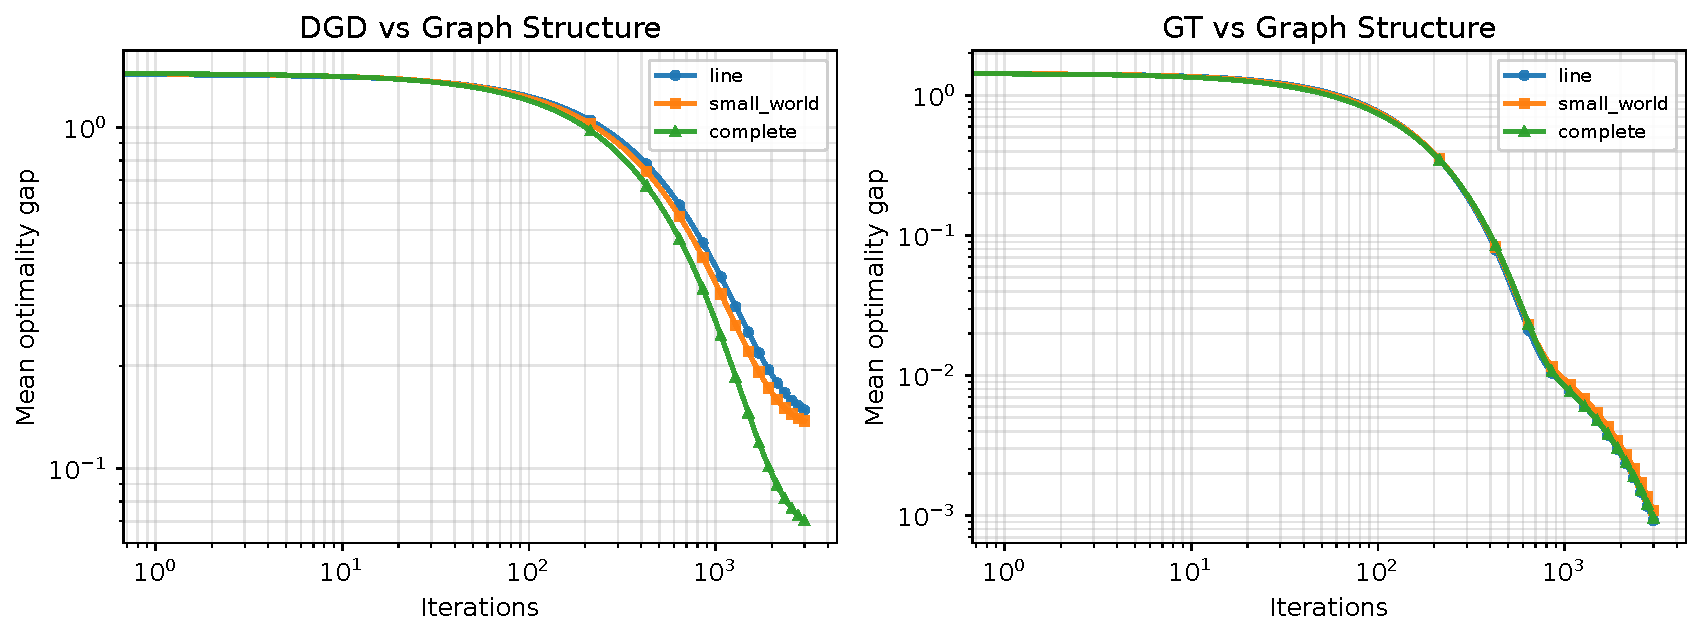
\includegraphics[width=\linewidth,trim=0 0 405 0,clip]{part1_graph_structure_comparison.pdf}
    \end{subfigure}\hfill
    \begin{subfigure}[t]{0.48\linewidth}
        \centering
        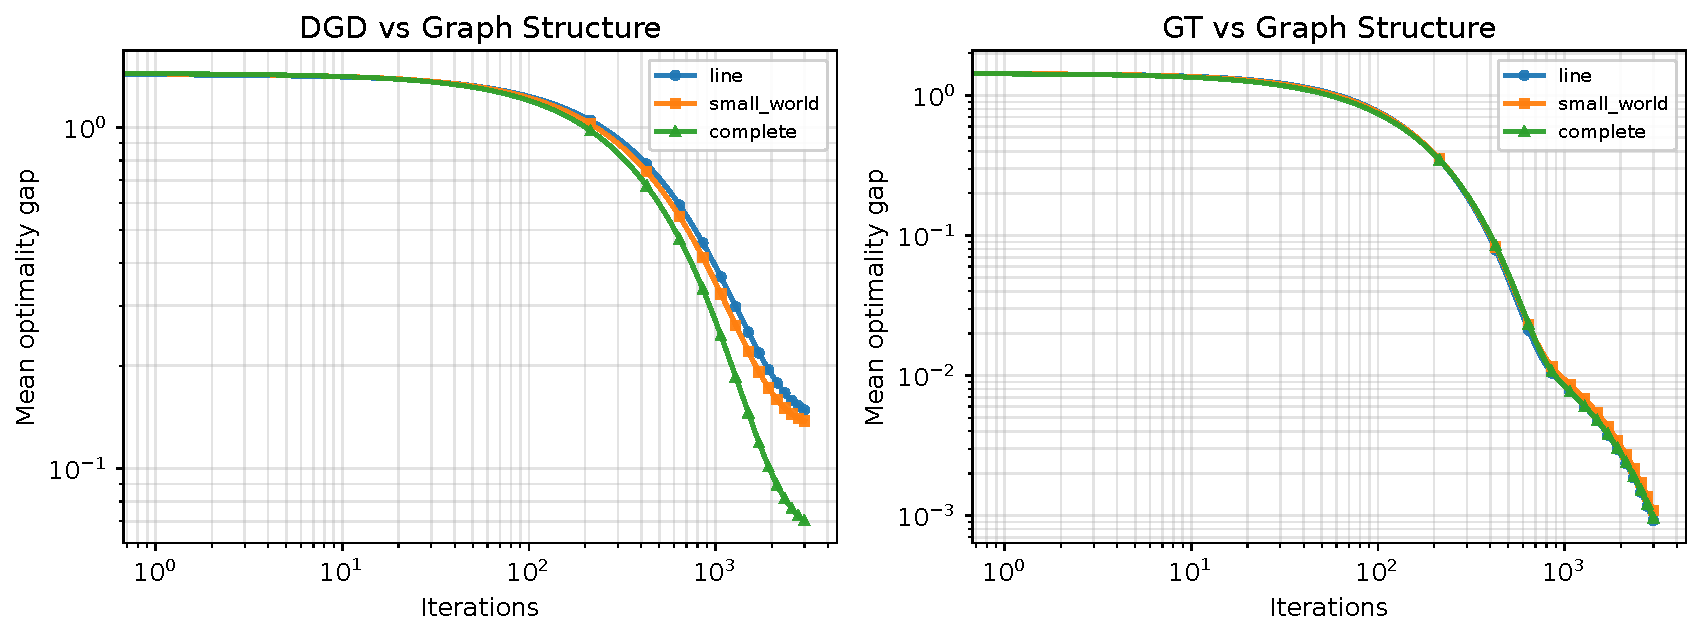
\includegraphics[width=\linewidth,trim=405 0 0 0,clip]{part1_graph_structure_comparison.pdf}
    \end{subfigure}
    \caption{Graph-topology comparison.}
    \label{fig:graph-topology}
\end{figure}

\paragraph{Directed communication, losses, and push-sum.}
Robustness beyond the symmetric connected setting is tested by introducing directed communication, packet losses, and asynchrony. Figure~\ref{fig:failures} isolates that experiment. Once the assumptions behind a symmetric doubly stochastic mixing matrix are violated, plain DGD degrades substantially. The directed-only curve and the directed-plus-loss-plus-asynchrony curve barely improve over the horizon. Push-sum, however, restores a stable descent profile in the directed case because it corrects the loss of average preservation induced by non-doubly-stochastic communication.

\paragraph{Trajectory scaling.}
The dependence on $n$ is examined under the rank rule $m=\lceil \sqrt{n}\rceil$. Figure~\ref{fig:scaling-trajectories} plots the $200$-step DGD trajectories for six problem sizes and should be read as a fixed-budget stress test. The curves initially improve as the model rank grows from the smallest regime, but the benefit disappears once the higher-dimensional consensus problem becomes too demanding for the fixed iteration budget.

\noindent
\begin{minipage}[t]{0.49\linewidth}
    \centering
    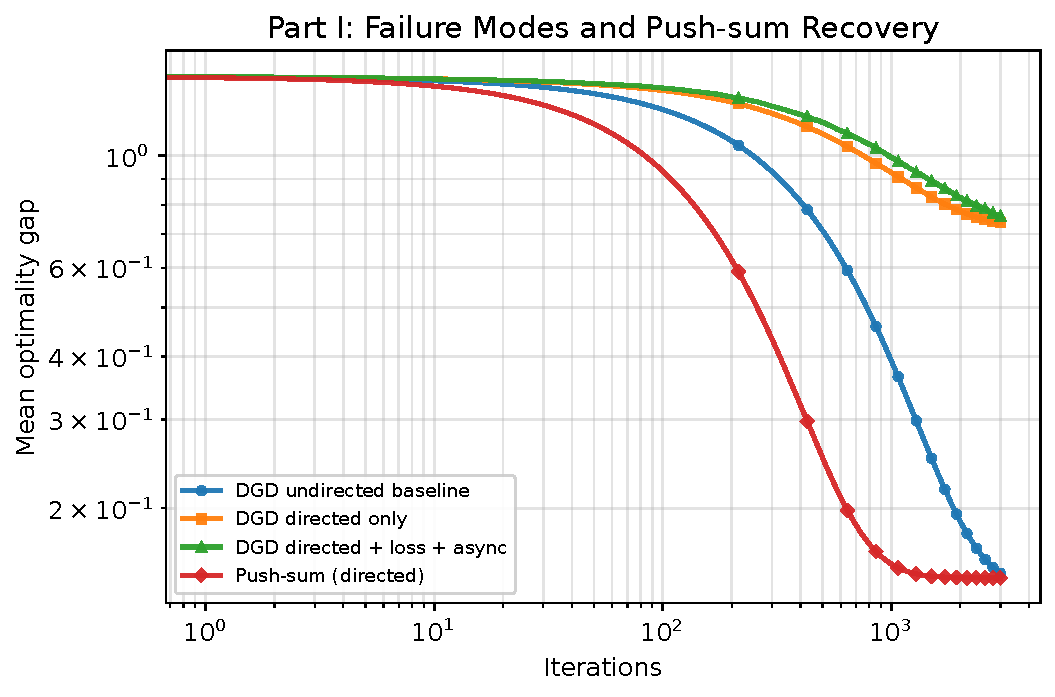
\includegraphics[width=\linewidth]{part1_failure_and_pushsum.pdf}
\par\smallskip
    \refstepcounter{figure}\label{fig:failures}
    {\small\textbf{Figure \thefigure.} Communication failures and push-sum recovery.\par}
\end{minipage}\hfill
\begin{minipage}[t]{0.49\linewidth}
    \centering
    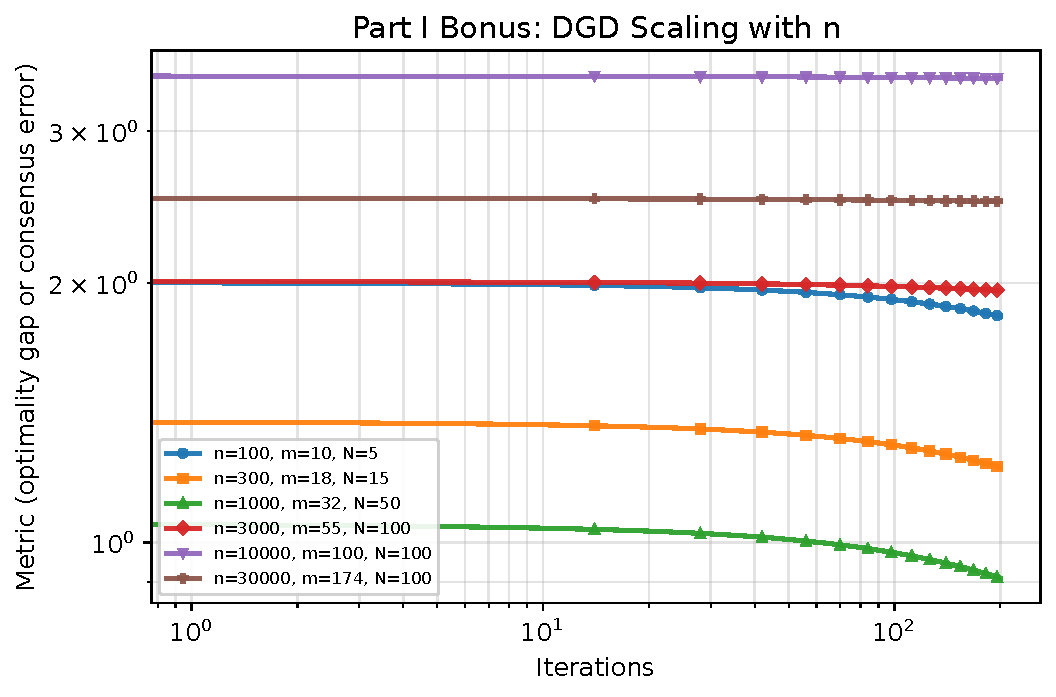
\includegraphics[width=\linewidth]{part1_bonus_scaling_convergence.pdf}
\par\smallskip
    \refstepcounter{figure}\label{fig:scaling-trajectories}
    {\small\textbf{Figure \thefigure.} Scaling trajectories.\par}
\end{minipage}

\paragraph{Endpoint statistics.}
Figure~\ref{fig:scaling-endpoints} compresses the same study into final metrics and runtimes. The final metric improves from \num{1.8296} at $n=100$ to \num{0.9098} at $n=1000$, but then worsens to \num{1.9603}, \num{3.4531}, and \num{2.4861} for $n=3000$, $10000$, and $30000$. At the same time the runtime grows from \num{1.88e-3}\,s to \num{9.57e-2}\,s (absolute times are machine dependent). The correct interpretation is not that larger problems are intrinsically impossible, but that a fixed $200$-iteration budget becomes insufficient once both the feature dimension and the network size are enlarged.

\begin{figure}[!htb]
    \centering
    \begin{subfigure}[t]{0.48\linewidth}
        \centering
        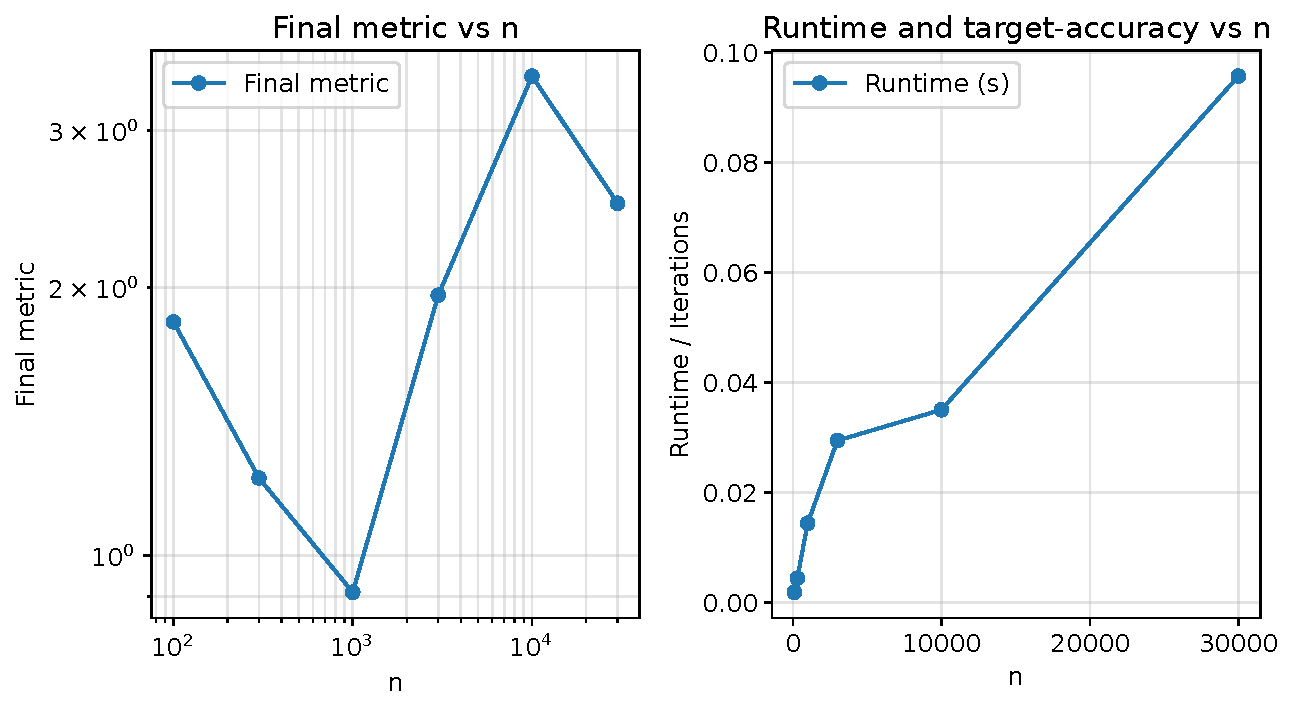
\includegraphics[width=\linewidth,trim=0 0 405 0,clip]{part1_bonus_n_dependency.pdf}
    \end{subfigure}\hfill
    \begin{subfigure}[t]{0.48\linewidth}
        \centering
        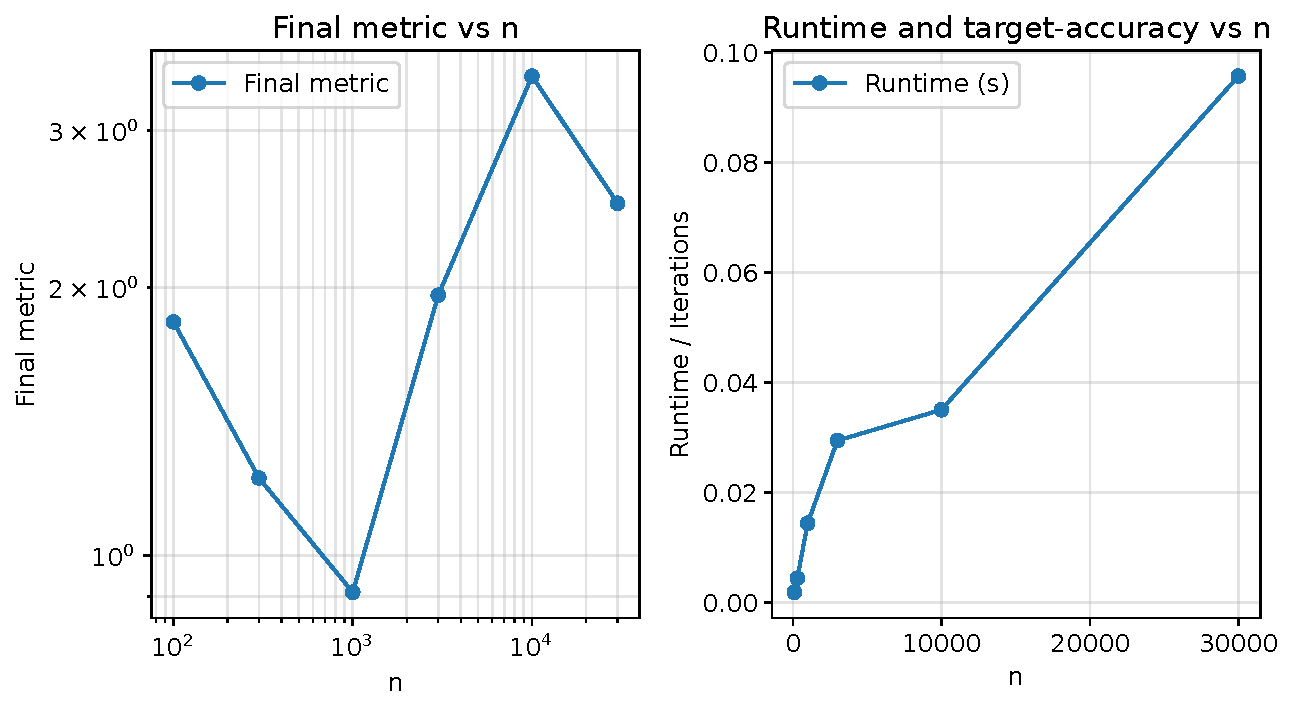
\includegraphics[width=\linewidth,trim=405 0 0 0,clip]{part1_bonus_n_dependency.pdf}
    \end{subfigure}
    \caption{Scaling endpoint statistics.}
    \label{fig:scaling-endpoints}
\end{figure}



\section{Federated Learning}\label{sec:federated}
\subsection{FedAvg model and learning rates}
The second dataset already comes partitioned into five local datasets $(X_c,Y_c)$. The server therefore does not access raw data and only aggregates model updates. In FedAvg, client $c$ starts round $t$ from the current server model $\alpha^t$ and performs $E$ local SGD epochs on batches of size $B$,
\begin{equation}
    \alpha_{c,\ell+1}=\alpha_{c,\ell}-\eta_t \nabla f_{B_\ell,c}(\alpha_{c,\ell}),
\end{equation}
after which the server computes the weighted average
\begin{equation}
    \alpha^{t+1}=\sum_{c\in S_t}\frac{n_c}{\sum_{j\in S_t} n_j}\,\alpha_{c,E}^{\,t}.
\end{equation}
Here $S_t$ is the set of selected clients and $n_c$ is the local sample count. In the experiments all clients have $n_c=20$, so the aggregation is uniform whenever the selected clients have equal size. The learning-rate audit in Table~\ref{tab:theory} gives $L_{\max}^{\mathrm{FL}}\approx\num{79.73}$ and confirms that the implemented initial rate $\eta_0=\num{0.002}$ is safely below the standard smooth convex reference bound \num{0.0251}.

\subsection{Objective-error comparisons}
\begin{figure}[!htb]
    \centering
    \begin{subfigure}[t]{0.48\linewidth}
        \centering
        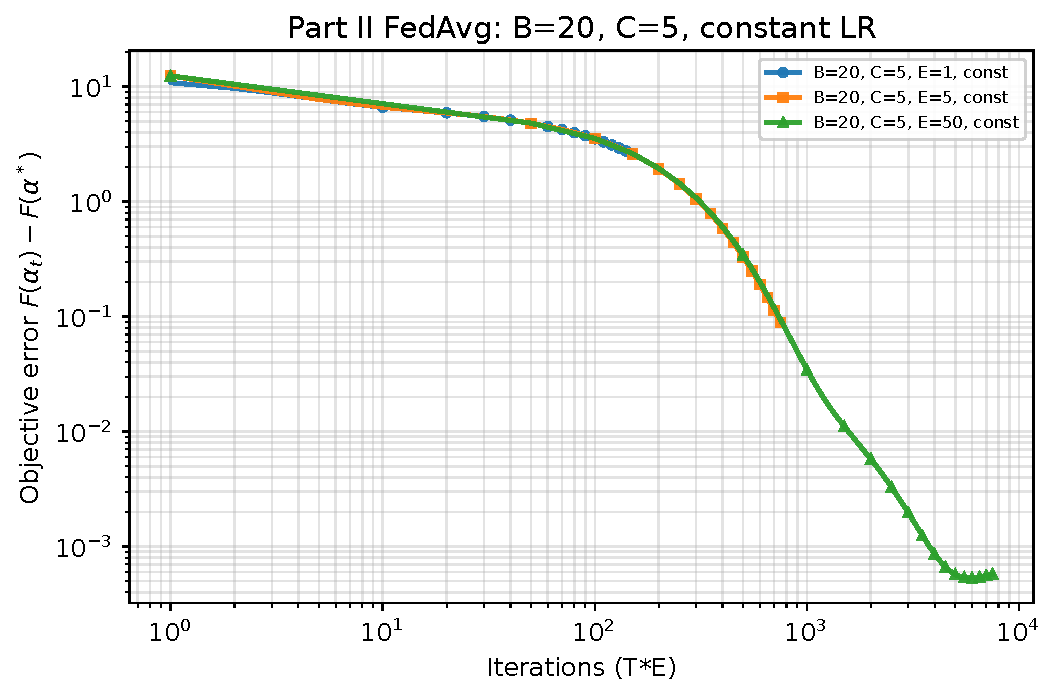
\includegraphics[width=\linewidth]{part2_fedavg_b20_c5_constant_lr.pdf}
    \end{subfigure}\hfill
    \begin{subfigure}[t]{0.48\linewidth}
        \centering
        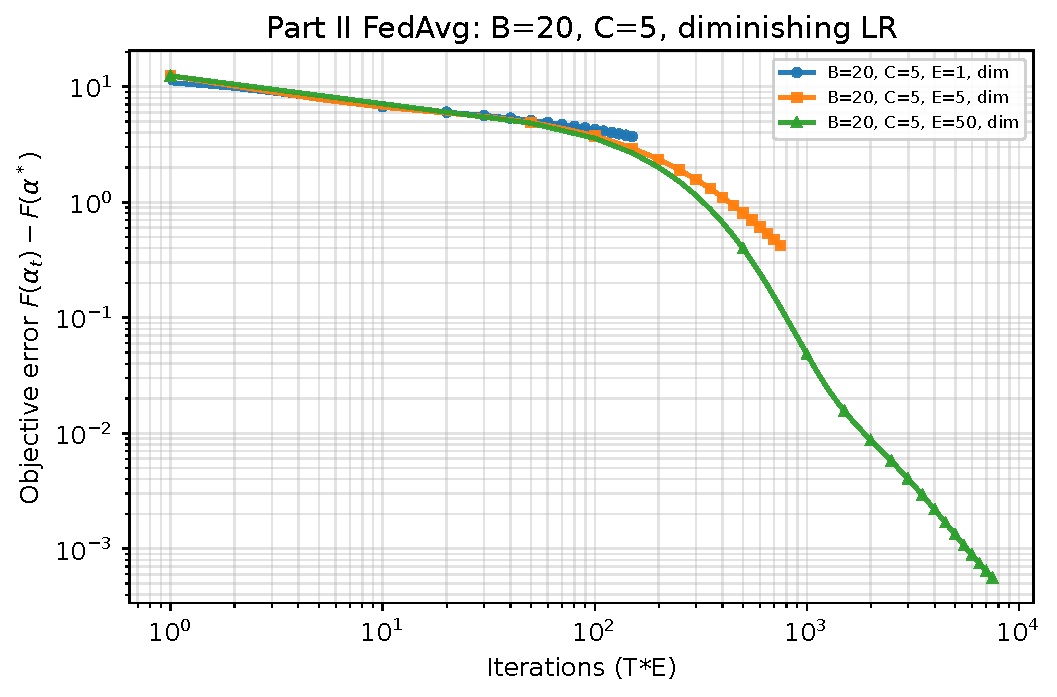
\includegraphics[width=\linewidth]{part2_fedavg_b20_c5_diminishing_lr.pdf}
    \end{subfigure}
    \caption{Baseline FedAvg experiments.}
    \label{fig:fedavg-mandatory}
\end{figure}
\paragraph{Baseline FedAvg behavior.}
The baseline federated experiments use $B=20$, $C=5$, and $E\in\{1,5,50\}$ under constant and diminishing learning rates. Figure~\ref{fig:fedavg-mandatory} reports the two corresponding plots. For the constant rate, increasing the local computation budget is uniformly beneficial: the final objective error drops from \num{2.5923} at $E=1$ to \num{8.8405e-2} at $E=5$ and to \num{5.7480e-4} at $E=50$. With the diminishing schedule, the initial progress is slower but the long-horizon behavior is slightly smoother, and the $E=50$ run ends at \num{5.5814e-4}. This is exactly the comparison predicted by the standard smooth-convex analysis: constant rates can perform very well at a finite horizon, whereas diminishing rates are the standard route to asymptotic accuracy.

\paragraph{Reduced batch size and client participation.}
Further comparisons vary the batch size and the number of participating clients. Figure~\ref{fig:fedavg-extra} isolates this effect within FedAvg. Lowering the batch size from $20$ to $15$ while keeping all five clients already worsens the best $E=50$ final error from \num{5.7480e-4} to \num{1.9502e-3}. Reducing the active clients to $C=3$ is much more damaging: the $B=15$, $C=3$, $E=50$ run finishes at \num{1.7102e-1}. These runs show that local computation alone is not enough; stable progress also depends on how much data each round actually aggregates.

\begin{figure}[!htb]
    \centering
    \begin{subfigure}[t]{0.48\linewidth}
        \centering
        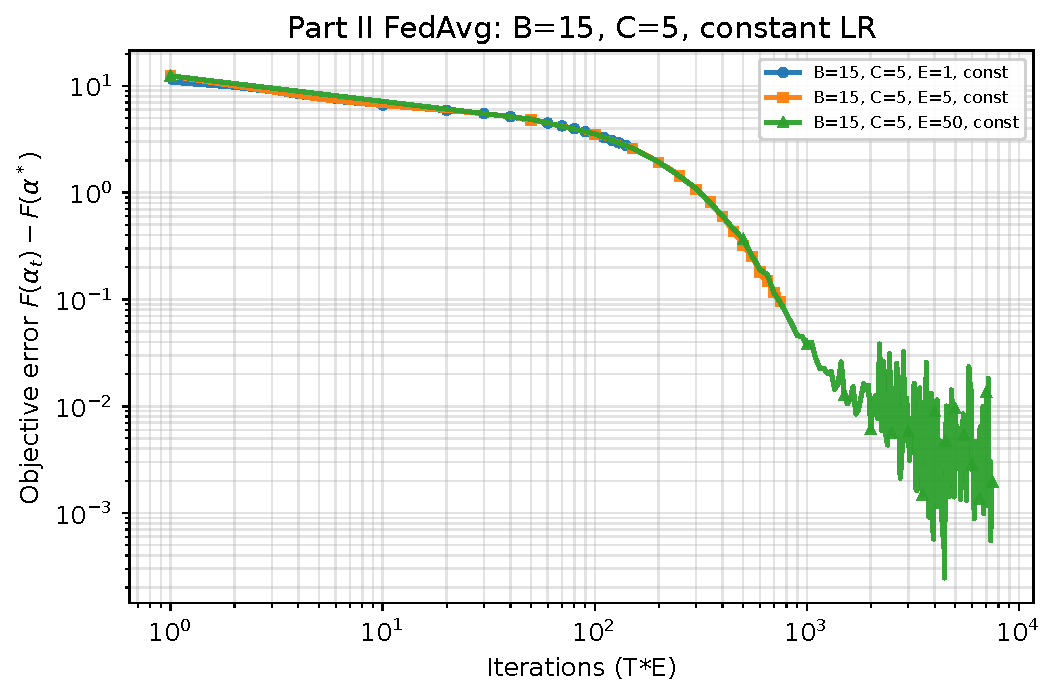
\includegraphics[width=\linewidth]{part2_fedavg_b15_c5_constant_lr.pdf}
    \end{subfigure}\hfill
    \begin{subfigure}[t]{0.48\linewidth}
        \centering
        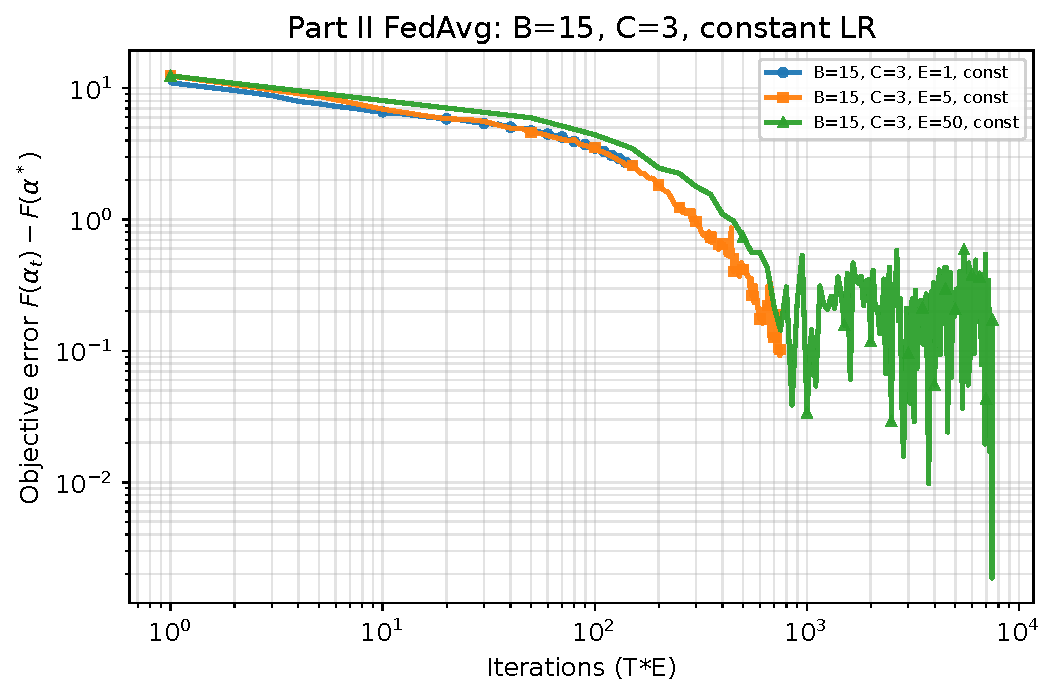
\includegraphics[width=\linewidth]{part2_fedavg_b15_c3_constant_lr.pdf}
    \end{subfigure}
    \caption{Reduced batches and client participation.}
    \label{fig:fedavg-extra}
\end{figure}

\paragraph{Control variates.}
The natural correction for client drift is SCAFFOLD, whose local update subtracts a client control variate and adds a global one,
\begin{equation}
    \alpha_{c,\ell+1}
    =
    \alpha_{c,\ell}
    -
    \eta\bigl(\nabla f_{B_\ell,c}(\alpha_{c,\ell})-h_c+h\bigr),
\end{equation}
so that client drift is corrected rather than merely averaged out at the server.

Figure~\ref{fig:scaffold} shows that control variates change the picture qualitatively. With SCAFFOLD, the method benefits from large local epoch budgets instead of drifting away from the global objective. At $E=50$, SCAFFOLD reaches \num{2.4461e-5} for $C=5$ and \num{2.3601e-5} for $C=3$, so even partial participation remains well controlled. This is consistent with a non-IID client partition, where plain FedAvg suffers from client drift.

\begin{figure}[!htb]
    \centering
    \begin{subfigure}[t]{0.48\linewidth}
        \centering
        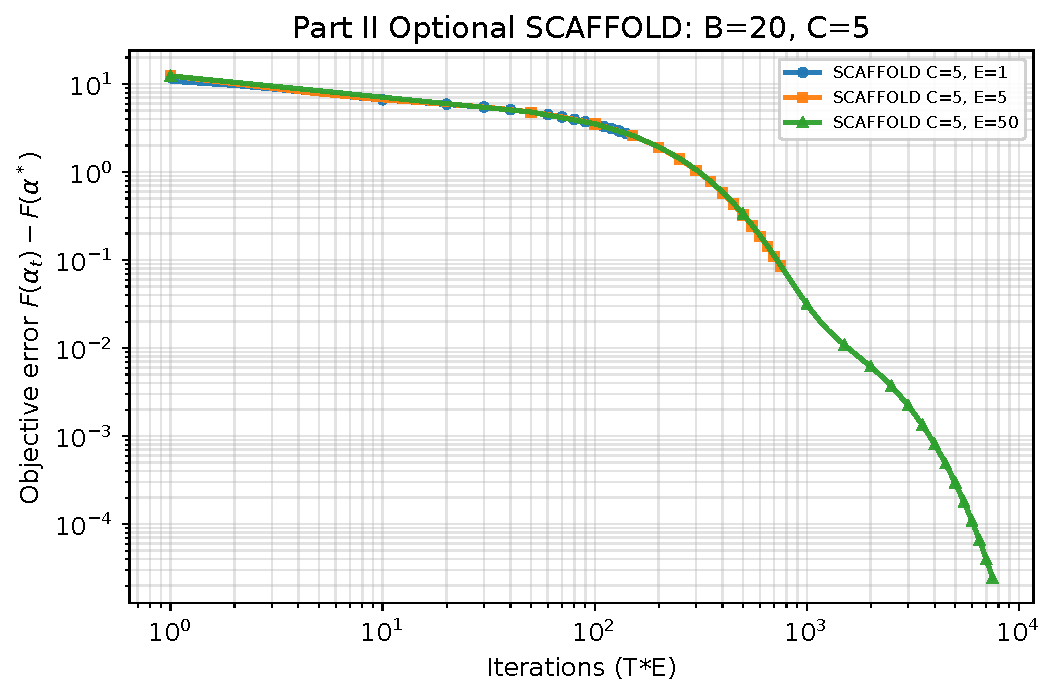
\includegraphics[width=\linewidth]{part2_scaffold_b20_c5.pdf}
    \end{subfigure}\hfill
    \begin{subfigure}[t]{0.48\linewidth}
        \centering
        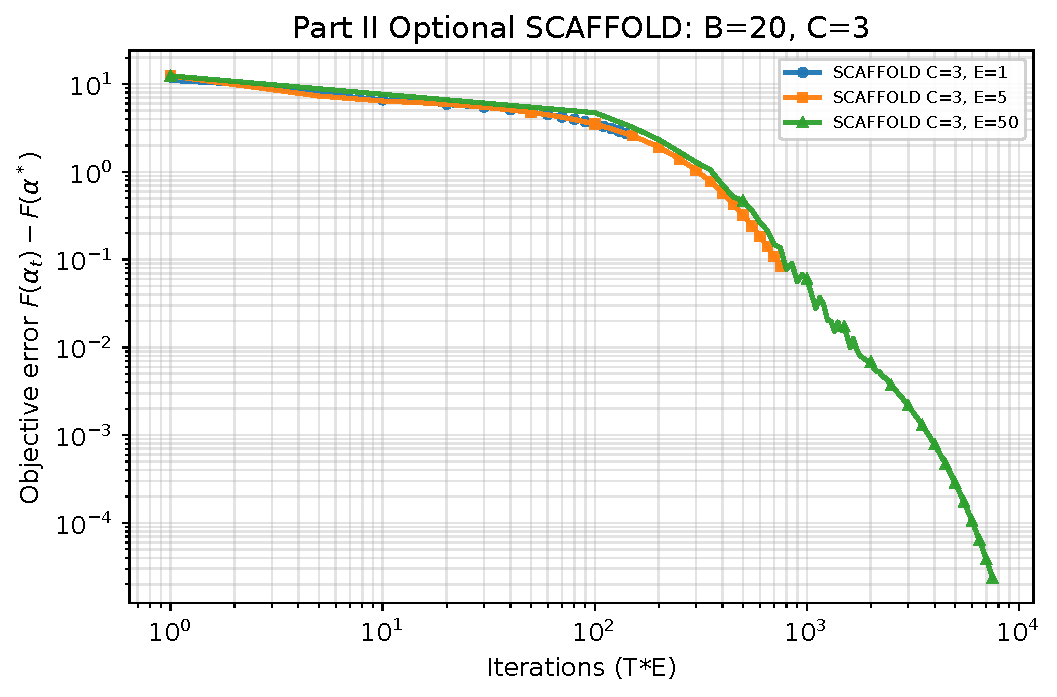
\includegraphics[width=\linewidth]{part2_scaffold_b20_c3.pdf}
    \end{subfigure}
    \caption{SCAFFOLD experiments.}
    \label{fig:scaffold}
\end{figure}

\FloatBarrier
\section{Differential Privacy}\label{sec:dp}
\subsection{Noisy consensus updates and schedule checks}
Part~III returns to the first dataset and perturbs inter-agent communication with Laplace noise. The implemented DP-DGD update follows the static-consensus construction studied in the course notes and in the supplied Wang--Nedi\'{c} paper. Each agent sends the noisy state $\chi_i^k = x_i^k + \zeta_i^k$ and performs
\begin{equation}
    x_i^{k+1}
    =
    x_i^k
    +
    \gamma_k\Bigl(\sum_{j=1}^a w_{ij}\chi_j^k - x_i^k - \alpha_k \nabla f_i(x_i^k)\Bigr),
\end{equation}
with schedules
\begin{equation}
    \alpha_k=\frac{0.002}{1+0.001k},\qquad
    \gamma_k=\frac{1}{1+0.001k^{0.9}},\qquad
    \nu_k=\frac{0.01}{\epsilon}\bigl(1+0.001k^{0.1}\bigr).
    \label{eq:dp-schedules}
\end{equation}
The parameter regime follows Theorem~2(3) of the supplied DP paper, while the course notes formulate the same summability conditions at the level of convergence and privacy bounds. The required asymptotic conditions are
\begin{equation}
    \sum_k \alpha_k = \infty,\qquad
    \sum_k \gamma_k = \infty,\qquad
    \sum_k \frac{\alpha_k^2}{\gamma_k} < \infty,\qquad
    \sum_k \frac{\alpha_k}{\nu_k} < \infty.
\end{equation}
The verification notes confirm that the implemented exponents satisfy these requirements. On the $3000$-step horizon used in the experiments, the audit gives $\sum_{k=1}^{3000}\alpha_k^2/\gamma_k=\num{4.2484e-3}$ and, for $\epsilon=1$, $\sum_{k=1}^{3000}\alpha_k/\nu_k=\num{2.7664e2}$. This does not by itself certify end-to-end differential privacy of the full experimental pipeline, but it does verify that the chosen schedules match the assumptions used by the theorems.

\subsection{Privacy--utility trade-off}
\paragraph{Baseline regime.}
The baseline trade-off is shown in the left panel of Figure~\ref{fig:dp-tradeoff}. The ranking is monotone in the privacy parameter, exactly as expected from the schedule \eqref{eq:dp-schedules}: smaller $\epsilon$ means larger noise variance and therefore a larger steady optimization error. The final gap is \num{0.2818} without privacy, then rises to \num{1.5882} for $\epsilon=10$, \num{2.7365} for $\epsilon=1$, and \num{12.3873} for $\epsilon=0.1$. The curves show that this is not only an endpoint effect. For the smallest $\epsilon$, the trajectory turns upward fairly early, meaning that the noise floor dominates the optimization progress well before the time horizon is exhausted.

\begin{figure}[!htb]
    \centering
    \begin{subfigure}[t]{0.45\linewidth}
        \centering
        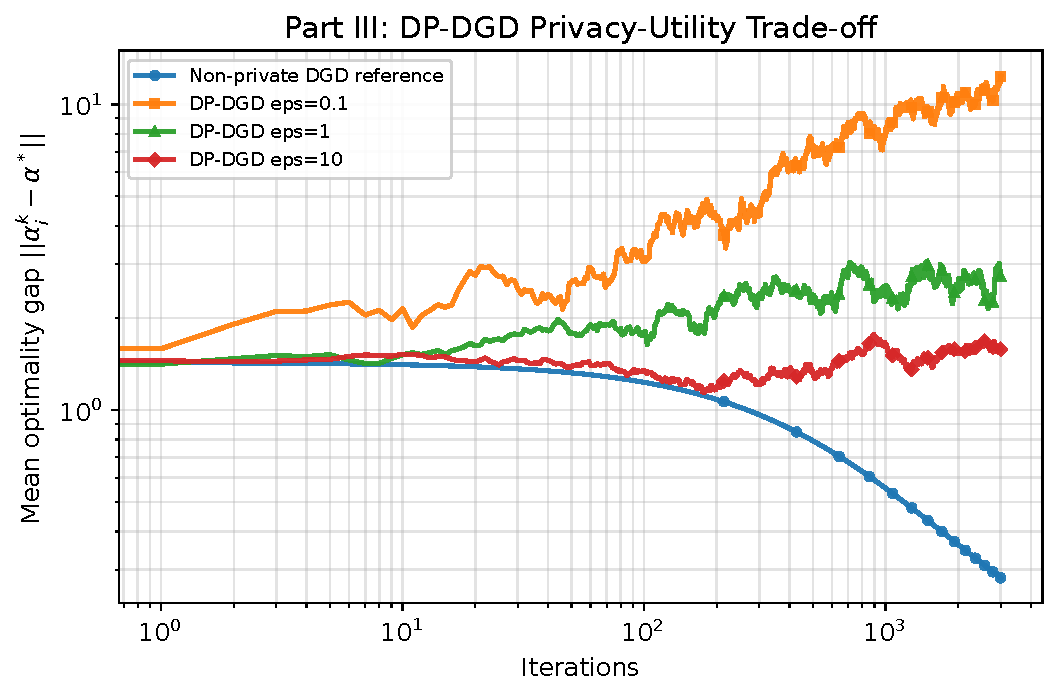
\includegraphics[width=\linewidth]{part3_dp_dgd_tradeoff.pdf}
    \end{subfigure}\hfill
    \begin{subfigure}[t]{0.45\linewidth}
        \centering
        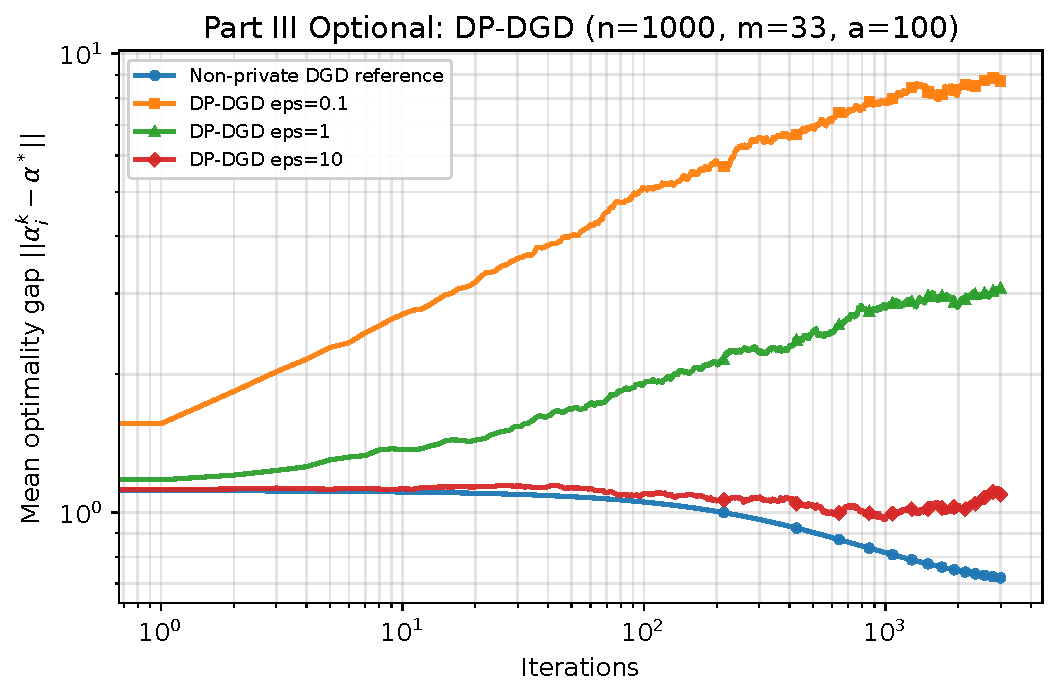
\includegraphics[width=\linewidth]{part3_optional_dp_dgd_tradeoff.pdf}
    \end{subfigure}
    \caption{DP-DGD under two problem sizes.}
    \label{fig:dp-tradeoff}
\end{figure}

\paragraph{Larger-scale extension and audit limits.}
The right panel of Figure~\ref{fig:dp-tradeoff} repeats the same experiment for $(n,m,a)=(1000,33,100)$. The qualitative picture is unchanged. The non-private reference ends at \num{0.7195}, while the private gaps become \num{1.0953}, \num{3.0812}, and \num{8.7693} for $\epsilon=10,1,0.1$. The larger-scale experiment therefore does not overturn the conclusions of the baseline one; it magnifies them by using a larger graph and a higher-dimensional model.

One caveat remains essential. The numerical audit reports empirical quantities under an \emph{unclipped bounded-sensitivity audit}. These diagnostics are useful for checking consistency with the theorem assumptions, but they are not a formal proof that every part of the experimental pipeline is rigorously private. The precise claim supported by the data is narrower: under the bounded-sensitivity assumption used by the implementation, the theorem-aligned schedules preserve the convergence pattern while exhibiting the expected privacy--utility degradation.

\FloatBarrier
\begin{table}[!htb]
\centering
\small
\renewcommand{\arraystretch}{1.03}
\setlength{\tabcolsep}{5pt}
\caption{Selected final metrics and runtimes.}
\label{tab:results}
\begin{tabular}{@{}l c r r@{}}
\toprule
Configuration & Metric & Final value & Runtime (s) \\
\midrule
\multicolumn{4}{@{}l}{\textit{Part I}} \\
DGD, line & Gap & \num{1.485e-01} & \num{2.641e-02} \\
GT, line & Gap & \num{8.592e-04} & \num{3.766e-02} \\
Dual dec., line & Gap & \num{4.137e-06} & \num{3.714e-02} \\
ADMM, $\beta=1$ & Gap & \num{1.995e-14} & \num{7.363e-02} \\
\addlinespace[2pt]
\multicolumn{4}{@{}l}{\textit{Part II}} \\
FedAvg $(20,5,50)$ const. & Obj. & \num{5.748e-04} & \num{1.940e-01} \\
FedAvg $(20,5,50)$ dim. & Obj. & \num{5.581e-04} & \num{1.963e-01} \\
FedAvg $(15,5,50)$ & Obj. & \num{1.950e-03} & \num{2.909e-01} \\
FedAvg $(15,3,50)$ & Obj. & \num{1.710e-01} & \num{1.638e-01} \\
SCAFFOLD $(20,5,50)$ & Obj. & \num{2.446e-05} & \num{2.084e-01} \\
SCAFFOLD $(20,3,50)$ & Obj. & \num{2.360e-05} & \num{1.262e-01} \\
\addlinespace[2pt]
\multicolumn{4}{@{}l}{\textit{Part III}} \\
Non-private DGD & Gap & \num{2.818e-01} & \num{3.670e-02} \\
DP-DGD, $\epsilon=10$ & Gap & \num{1.588e+00} & \num{5.380e-02} \\
DP-DGD, $\epsilon=1$ & Gap & \num{2.737e+00} & \num{5.352e-02} \\
DP-DGD, $\epsilon=0.1$ & Gap & \num{1.239e+01} & \num{5.386e-02} \\
\addlinespace[2pt]
\multicolumn{4}{@{}l}{\textit{Part III ext.}} \\
Non-private DGD & Gap & \num{7.195e-01} & \num{8.198e-01} \\
DP-DGD, $\epsilon=10$ & Gap & \num{1.095e+00} & \num{1.241e+00} \\
\bottomrule
\end{tabular}
\end{table}

\FloatBarrier
\vspace{-0.4em}

\section{Conclusion}
Taken together, the experiments show a consistent picture. In distributed optimization, exact-consensus methods dominate DGD on the quadratic kernel model: ADMM is the most accurate baseline solver, dual decomposition is the next best exact method, and GT removes the nonzero error floor of DGD. In federated learning, larger local epoch budgets are highly effective once the learning rate is controlled, but heterogeneity makes plain FedAvg fragile when batches or participating clients are reduced; SCAFFOLD corrects that drift. In the private setting, the theorem-aligned schedules remain numerically consistent with the convergence and privacy assumptions, but stronger privacy worsens the optimization gap. The large-$n$ study should be read as a fixed-budget stress test, and the privacy discussion remains an empirical audit rather than a full certification.

\end{document}
